\chapter{Introduction}

%%%%%%%%%%%%%%%%%%%%%%%%%%%%%%%%%%%%%%%%%%%%%%%%%%%%%%%%%%%%%%%%%%%%%%%%%%%%%%%%%%
%%%%%%%%%%%%%%%%%%%%%%%%%%%%%%%%%%%%%%%%%%%%%%%%%%%%%%%%%%%%%%%%%%%%%%%%%%%%%%%%%%
%                Section: Spatial Data and Predictands
%%%%%%%%%%%%%%%%%%%%%%%%%%%%%%%%%%%%%%%%%%%%%%%%%%%%%%%%%%%%%%%%%%%%%%%%%%%%%%%%%%
%%%%%%%%%%%%%%%%%%%%%%%%%%%%%%%%%%%%%%%%%%%%%%%%%%%%%%%%%%%%%%%%%%%%%%%%%%%%%%%%%%

\section{Spatial Data and Predictands}

The types of spatial data considered in this book have basic form
\[ \{(S_i,y_i):i=1,\ldots,n\}, \]
where $S_i$ is a ``site" (spatial location) in a spatial domain ${\cal A}$ of interest and $y_i$ is the observed value of a real-valued ``response" variable $y$ at $S_i$.  Typically, the $S_i$'s are distinct, i.e., there is only one observation taken at each site, but this is not strictly required.  The spatial domain ${\cal A}$ is usually a region within $\mathbb{R}^d$, where $d=1$, 2, or 3 and is often Euclidean, but again this is not strictly required; non-Euclidean spatial domains of considerable interest include the surface of a sphere (such as one that approximates the earth's surface) or a spatial network (such as a river network).  A vector ${\bf z}_i$ of ``covariates" (additional variables that may help to explain the response) may also be observed at each site, in which case the basic form of the data is expanded to $\{(S_i,y_i,{\bf z}_i):i=1,\ldots,n\}$.  It is also possible that the response is multivariate rather than univariate, in which case the scalar $y_i$ in these data representations is replaced with a vector ${\bf y}_i$ of response variables observed at $S_i$.   

The term ``site" in the preceding paragraph is intentionally imprecise, so as to encompass the two types of spatial data commonly known as {\em areal data} and {\em geostatistical data}.  Areal data are observations taken at nonoverlapping, contiguous (or nearly so) subregions $\{A_i:i=1,\ldots,n\}$ of ${\cal A}$.  The subregions have well-defined boundaries, which may be regularly or irregularly shaped.  Such data often arise by counting discrete events (e.g.\ disease cases) within administrative units (such as counties or wildlife management units), or by averaging a continuous variable (e.g. soil moisture) over well-defined areas (such as field plots or watersheds).  Geostatistical data, like areal data, are taken at sites that are nonoverlapping subregions, but in contrast to areal data, the subregions are not contiguous and are so small relative to the spacing between them that nothing of consequence is lost by idealizing them as individual points $\{{\bf s}_i: i=1,\ldots,n\}$, one representing each subregion.  Such data are often measurements of a continuous variable at a particular time or aggregated over time, such as the maximum ozone level recorded on a particular day at each monitoring site in a network of such sites distributed throughout a large city, or annual rainfall amounts at a network of rain gauges in a given year.

The following are introductions to four spatial datasets, two areal and two geostatistical, that will be featured throughout this book.
%------------------------------------------------------------------------------
%       Example 1.1.  Trends in harbor seal abundance
%------------------------------------------------------------------------------
\vspace{.25in}
\newline
\begin{tcolorbox}
{\bf Example 1.1.  Trends in harbor seal abundance}
\end{tcolorbox}
\vspace{.1in}
\begin{figure}
\begin{center}
\includegraphics[width=0.6\textwidth]{Chapter1/figure/seal_Stocks-crop.pdf}
\caption{Polygons where harbor seals occur. The upper right corner shows a map of Alaska, USA, and the study area, known as Southeast Alaska, is outlined in red. All polygons encapsulate coastal rocks along the mainland, or around islands, where seals hauled out and were counted.  There are 12 seal stocks (genetically distinct populations) along the southern coast of Alaska, and stocks 8 -- 12 occur in Southeast Alaska.  The set of polygons forming the geographic range of each stock is labelled and shown as a distinct color.
\label{fig:sealStocks}}
\end{center}
\end{figure}
%
Our first example is an areal data set of harbor seal trends \citep{ver2018spatial}. Figure \ref{fig:sealStocks} is a map showing Southeast Alaska, USA, in the upper right, and the study area outlined in red. Harbor seals haul out on rocks along the coast, but the exact rocks that they use change somewhat from survey to survey. Hence, 463 sample units, as polygons, were created so that counts of harbor seals could be obtained from any rocks they might use within the polygons. The polygons encapsulate all known seal haulouts from more than 30 years of monitoring.  The harbor seal population in Alaska extends from the Aleutian Islands in the west, to Southeast Alaska, and has been divided into 12 stocks (genetically distinct populations).  Five of the stocks, numbered 8 -- 12, are shown in Figure \ref{fig:sealStocks}. Seals were counted at various intensities (from 0 to 6 times per year per polygon) from aerial surveys over a 14-year period. Using counts as the response variable, trends for most polygons were estimated using Poisson regression (with year as the independent variable). To eliminate the effect of small sample sizes and imprecise estimates, polygons with fewer than two surveys over the 14-year period were eliminated, along with trends (linear on the log scale) that had estimated variances greater than 0.1. For demonstration purposes, we ignored the estimated variances and treated the estimated trends, on the log scale, as raw data.  Those estimated trends are shown in Figure \ref{fig:sealTrends}.
%
\begin{figure}
\begin{center}
\includegraphics[width=0.6\textwidth]{Chapter1/figure/seal_Trends-crop.pdf}
\caption{Map of raw seal trends in Southeast Alaska.  Colors show the magnitude of the estimated trends.  Each polygon is colored, but because some polygons are small and difficult to see, a circle was plotted over the centroid of each polygon and given the same color. Polygons colored by grey have missing data.
\label{fig:sealTrends}}
\end{center}
\end{figure}
%
Some polygons had missing data, having fewer than two total surveys, or an estimated variance of greater than 0.1, resulting in 306 polygons with estimated trends and 157 that were missing. A common way to model autocorrelation for areal data, such as these, is by using the idea of neighbors. When sample units are relatively large polygons, distance between them is not well defined, as distance could be between the closest two points from each polygon, the centroids of each polygon, etc.  Using the idea of neighbors is a flexible way to form associations, such as those that share a boundary or touch in some way (this can also be used in non-spatial situations such as social networks). Figure \ref{fig:sealNeighbors}A shows neighbors that we defined for this study area, which are largely those that touch (with a few isolated polygons joined to its nearest neighbor). The definition of neighbor can be flexible, so in Figure \ref{fig:sealNeighbors}B we included the neighbors of neighbors found in Figure \ref{fig:sealNeighbors}A.  Figure \ref{fig:sealNeighbors}B zooms into the area colored in gray in Figure \ref{fig:sealNeighbors}A, as otherwise too much detail is lost. Figure \ref{fig:sealNeighbors}B can be thought of as second-order neighbors. Figure \ref{fig:sealNeighbors}C, which can be thought of as fourth-order neighbors, includes the neighbors of neighbors found in Figure \ref{fig:sealNeighbors}B.
\begin{figure}
\begin{center}
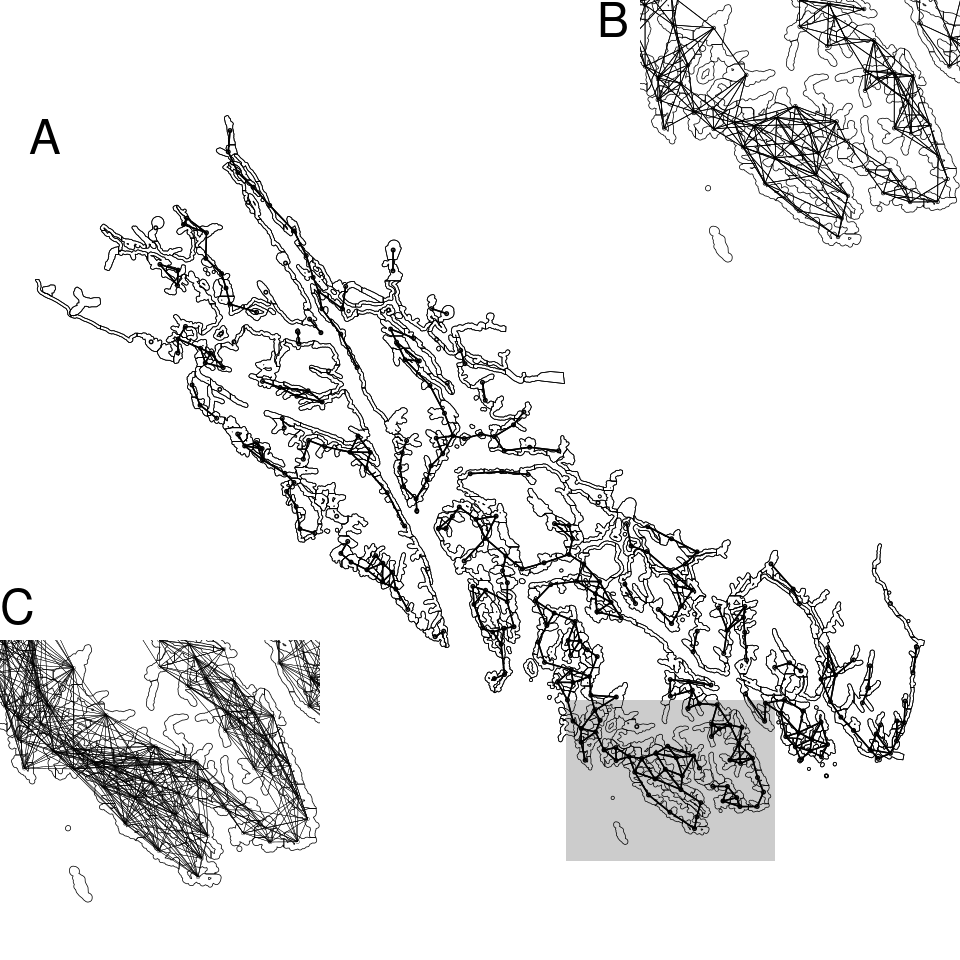
\includegraphics[width=0.6\textwidth]{Chapter1/figure/seal_Neighbors.pdf}
\caption{Map showing neighbors for harbor seal data. Lines connecting polygons indicate that they are neighbors.  A) First-order neighbors. Generally, defining neighbors means that polygons share at least one point in common.  In cases of isolated polygons, the nearest polygon, based on centroids, was used. B) Second-order neighbors.  These include the neighbors of the neighbors for first-order polygons.  C) Fourth-order neighbors.  These include the neighbors of the neighbors for second-order polygons.
\label{fig:sealNeighbors}}
\end{center}
\end{figure}

Some questions that an analysis of these data should attempt to address are as follows:
\begin{itemize}
\item Are there differences in trends among the 5 stocks?
\item Is there spatial dependence in the data, given that we have estimated an effect for each stock? Another way to think of this is as ``residual spatial autocorrelation.''
\item If there is residual spatial autocorrelation, must we account for it?  That is, how does it affect our trend estimates?
\item Which is a better model for residual spatial autocorrelation, the first-order, second-order, or fourth-order neighborhood structure?  How can we decide among them?
\item Can we make predictions, along with uncertainty intervals, for polygons with missing data?
\item Can we smooth over the observed data to reveal localized areas of increasing and decreasing trends?
\end{itemize}

$\quad\blacksquare$
\vspace{.5in}

%------------------------------------------------------------------------------
%             Caribou forage experiment
%------------------------------------------------------------------------------
\begin{tcolorbox}
{\bf Example 1.2.  Caribou forage experiment}
\end{tcolorbox}
\vspace{.1in}

Global climate change is expected to have consequences for ecosystems.  Caribou are adapted to certain vegetation, and may be limited by the amount and nutrition of their forage as climates change. An experiment was designed in Alaska to determine what factors might affect plant nutrition in the summer range of caribou. Details of the study and data are given in \citet{lenart2002climate}. A $5 \times 6$ grid of plots, where each plot was 1.8 by 3.6 m, was spaced 7.5 m horizontally and 9.8 m vertically (Figure \ref{fig:caribouDesign}).  Plots were covered with a clear tarp (to create increased temperature and less moisture), a shade tarp (to create cooler and somewhat drier conditions, as the tarp allowed some light and moisture to pass through), or plots were left uncovered.  To separate the moisture effect, water was added, or left untreated, as an additional main effect, creating 6 combinations of tarp and added moisture.  In a classical designed experiment, this is a two-factor design, and it can allow for interactions between the factors.  The treatments were established in two years, 1994 and 1995. Each plot had 8 subplots. One subplot was clipped during green-up, late spring, peak biomass, and senescence time periods in each year, so all 8 plots were eventually clipped. Plant material was separated into graminoids, forbs, and prostrate willows.  Nitrogen is a critical component of caribou diet, and percent nitrogen was provided by laboratory analyses for each sample. We focus on percent nitrogen in prostrate willows in the 3rd clipping (peak biomass) of the second year (to capture any accummulated effects).  These data are categorized into 4 color classes in Figure \ref{fig:caribouDesign}.  
%
\begin{figure}
\begin{center}
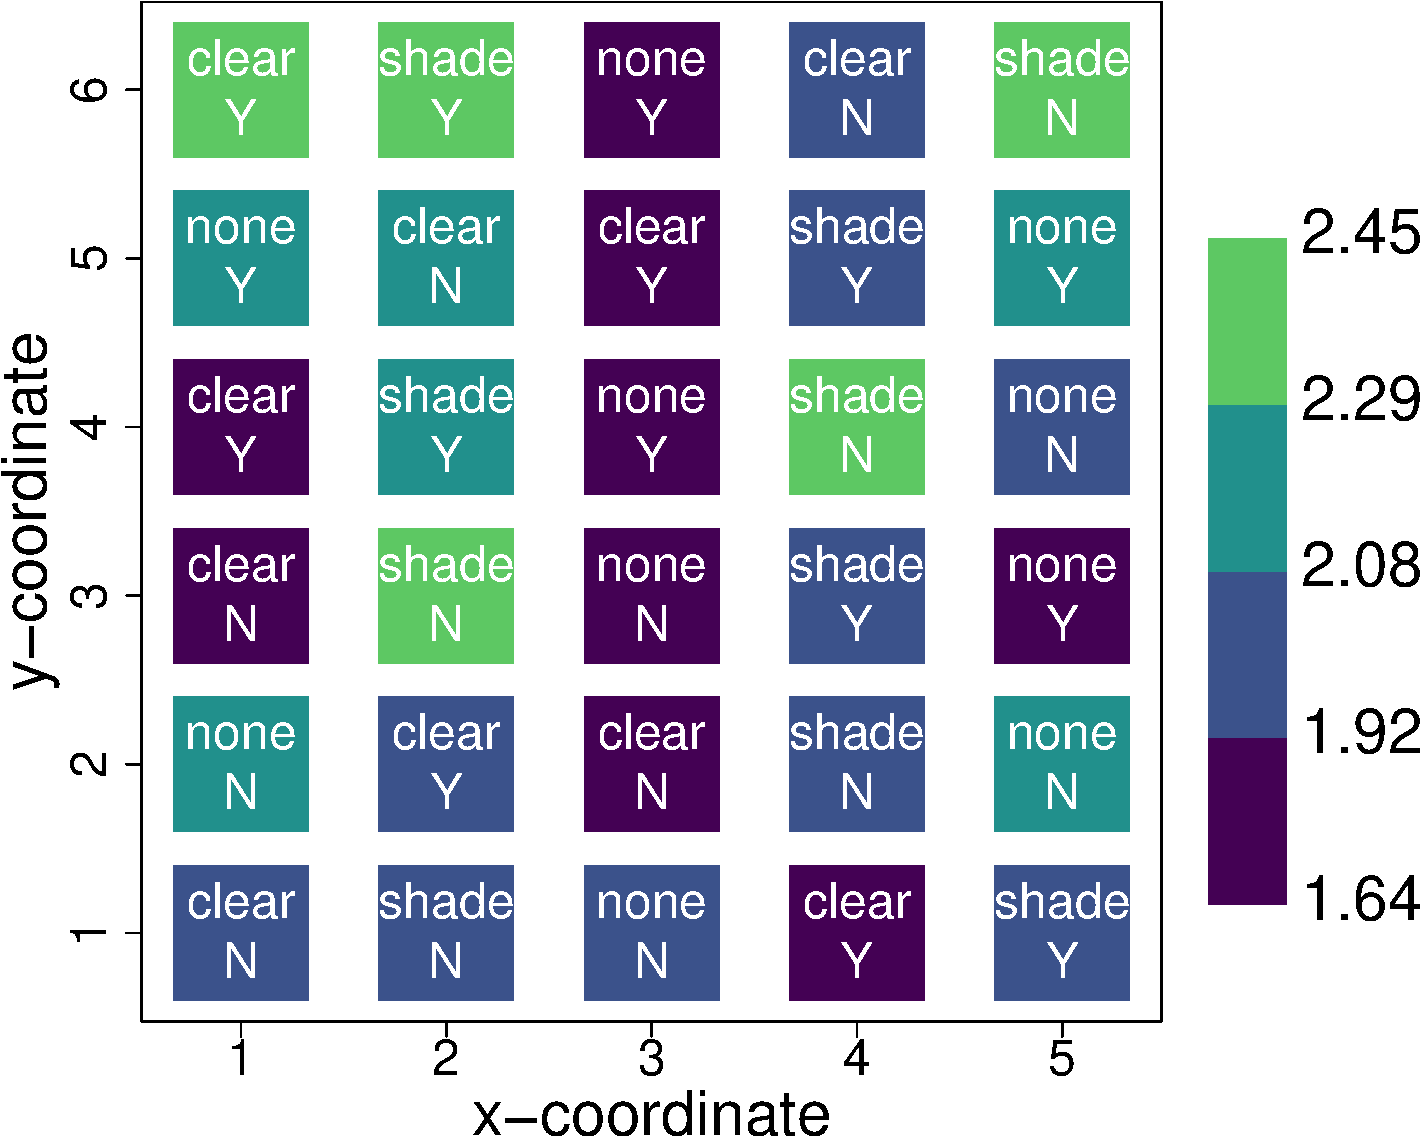
\includegraphics[width=0.6\textwidth]{Chapter1/figure/caribou_Design.pdf}
\caption{Designed experiment to determine how climate might affect forage biomass for caribou.  There were two treatment factors: 1) a tarp over the plot, which could be either clear, shade, or none, and 2) adding water, which could be yes or no.  The response to each treatment combination is colored, with the legend on the right giving the values for each color class.  In the plots themselves, the upper label is the tarp treatment, and the lower label is the water treatment, where Y indicates water added, and N indicates no water added.
\label{fig:caribouDesign}}
\end{center}
\end{figure}
%
Boxplots of percent nitrogen in prostate willows, for the third clipping in the second year, for the 6 treatment combinations, are shown in Figure \ref{fig:caribouBoxplots}.
%
\begin{figure}
\begin{center}
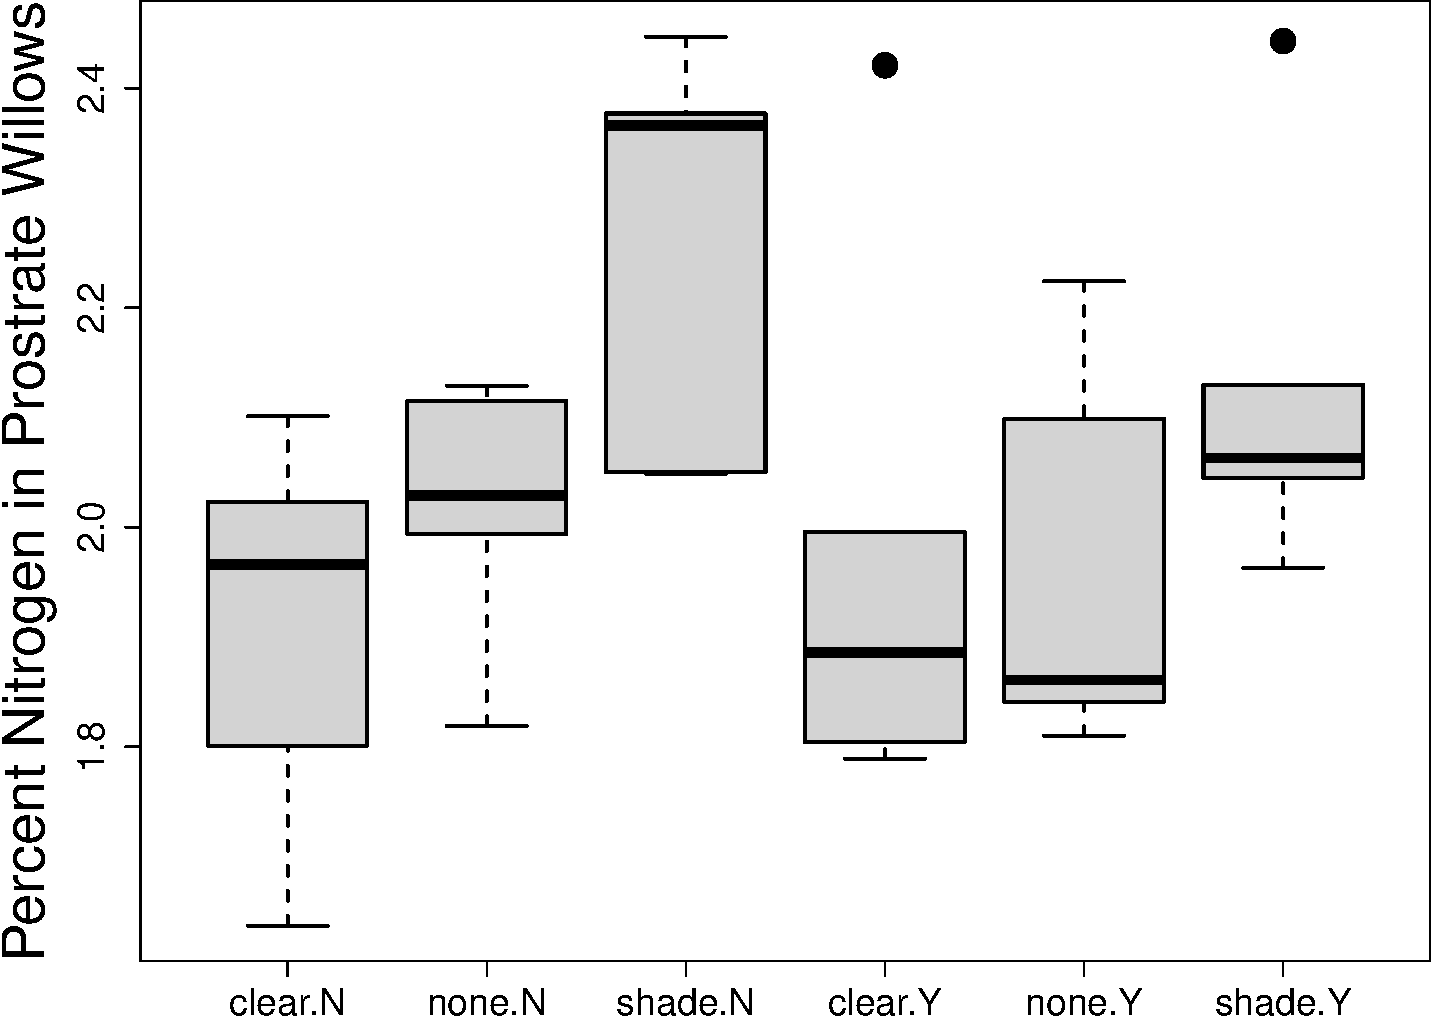
\includegraphics[width=0.6\textwidth]{Chapter1/figure/caribou_boxplots.pdf}
\caption{Boxplots of percent nitrogen in prostrate willows during the third clipping (peak biomass) of the second year of treatments.  Below each boxplot, ``clear'', ``none'', and ``shade'' indicate the tarp treatment, followed by the water treatment after the dot, where ``Y'' indicates water was added, and ``N'' is the control.
\label{fig:caribouBoxplots}}
\end{center}
\end{figure}
%

Some questions that we might ask of these data are as follows:
\begin{itemize}
\item Is there a significant difference among the tarp treatments, and which one provided the highest nitrogen percentage?
\item Is there a significant difference when adding water to the plots?  
\item Is there an interaction effect, where water added to clear tarps makes more difference than water added to shade or no tarp?
\item After accounting for the treatment effects, is there still spatial dependence in the data, and if so, must we account for it?  That is, how does residual spatial autocorrelation affect our estimates of the treatments?
\item What should we consider as our neighborhood structure for residual spatial autocorrelation?  Should we try several, and how can we decide among them?
\item While these data fit our conceptual framework for areal data, the nice regular grid also allows us to use distance among plots (centroid to centroid) to model autocorrelation (geostatistical models).  How might that compare to using neighborhood models for areal data?
\end{itemize}

$\quad\blacksquare$
\vspace{.5in}

%------------------------------------------------------------------------------
%            Example 1.3. Wet sulfate deposition
%------------------------------------------------------------------------------
\begin{tcolorbox}
{\bf Example 1.3. Wet sulfate deposition}
\end{tcolorbox}
\vspace{.1in}

Figure \ref{fig:SO4Intro} is a map showing total wet sulfate (SO$_4$) deposition amounts (in grams per square meter) for 1987, at locations of 198 sites in the continental United States that were part of the National Atmospheric Deposition Program/National Trends Network (NADP/NTN) and met quality assurance criteria in that year.  Deposition amounts of several ion species were recorded weekly at sites but we focus only on sulfate and  aggregate the weekly amounts into an annual total here.  No covariates were measured.  Thus, in terms of the notation introduced earlier, ${\cal A}$ is the continental United States and $S_i$ is the subregion occupied by the bucket that collects precipitation.  It is obvious from the map that the distances separating the buckets are very large relative to the size of the buckets, so it is reasonable to regard the data as geostatistical with point sites ${\bf s}_1,\ldots,{\bf s}_n$ giving the (longitude, latitude) coordinates of each NADP/NTN site.  Strictly, in this case ${\cal A}$ is not Euclidean; however, one might argue that the curvature of the earth over the continental United States is sufficiently small that a planar projection, such as Albers equal area projection \citep{snyder1987map}, shown in Figure 1.1, adequately represents the spatial information in the data.
\begin{figure}
\begin{center}
\includegraphics[width=0.6\textwidth]{Chapter1/figure/SO4_Intro-crop.pdf}
\caption{Map of wet sulfate deposition data locations, where color classes indicate annual rates of deposition.  The legend shows the break points between color classes.
\label{fig:SO4Intro}}
\end{center}
\end{figure}

%\begin{figure}
%\begin{center}
%\includegraphics[width=0.8\textwidth]{167so4.pdf}
%\caption{Three-dimensional scatterplot of wet sulfate deposition data.}
%\end{center}
%\end{figure}

Some questions that an analysis of these data should attempt to address are as follows:
\begin{itemize}
\item Where in the United States is wet sulfate deposition greatest?  Where is it so small as to be of no concern?
\item Is the wet sulfate deposition surface of the United States ``smooth" or do some sites have unusually high levels relative to nearby sites?
\item Is there spatial dependence in the data, and if so, at what scale does it exist?
\item Does the answer to the previous question depend on direction, i.e., on the relative orientation of sites?
\item Can we predict what the contemporaneous sulfate deposition was at an arbitrary unsampled location, or averaged over a selected subregion?
\end{itemize}
$\quad\blacksquare$
\vspace{.5in}

%------------------------------------------------------------------------------
%          Example 1.4.  Heavy metal concentrations in mosses
%------------------------------------------------------------------------------
\begin{tcolorbox}
{\bf Example 1.4.  Heavy metal concentrations in mosses}
\end{tcolorbox}

Figure \ref{fig:RedDogMap} is a map of Cape Krusenstern National Park in Alaska. To the north and east of Cape Krustenstern is the Red Dog mine, which is the United States' largest source of zinc. Other heavy metals, such as lead and cadmium, are also mined there. A haul road from the Red Dog Mine traverses Cape Krusenstern to the coast. Trucks haul ore to the coast to be barged away during the short Alaskan summers.  It is theorized that dust escapes into the environment from trucks. Mosses obtain much of their nutrients from the air, so they are ideal biomonitors for dust laden with heavy metals that mosses absorb.  In 2001 \citep{hasselbach2005spatial} and again in 2006 \citep{neitlich2017trends} mosses were sampled for heavy metals, with sampling more dense near the road (Figure \ref{fig:RedDogSampling}A).  Moss tissue samples were collected by snipping current annual growth, and then this was ground and homogenized before sending it out for laboratory analysis. Here, we just consider zinc concentrations, although many other elements were analyzed. While we will have many of the same goals as for Example 1.3, here we have important covariates, including distance from haul road, side of the road (north or south), year of sample, elevation, slope, and aspect.  Figure \ref{fig:RedDogDistRoad} shows higher concentrations of zinc near the road, for both years 2001 and 2006, with possible differences in the relationship on the north side of the road versus the south side, and possible differences by year as well.   

\begin{figure}
\begin{center}
\includegraphics[width=0.6\textwidth]{Chapter1/figure/RedDog_Alaska-crop.pdf}
\caption{Map showing the location of Cape Krusenstern National Park in Alaska, outlined in red.\label{fig:RedDogMap}}
\end{center}
\end{figure}

\begin{figure}
\begin{center}
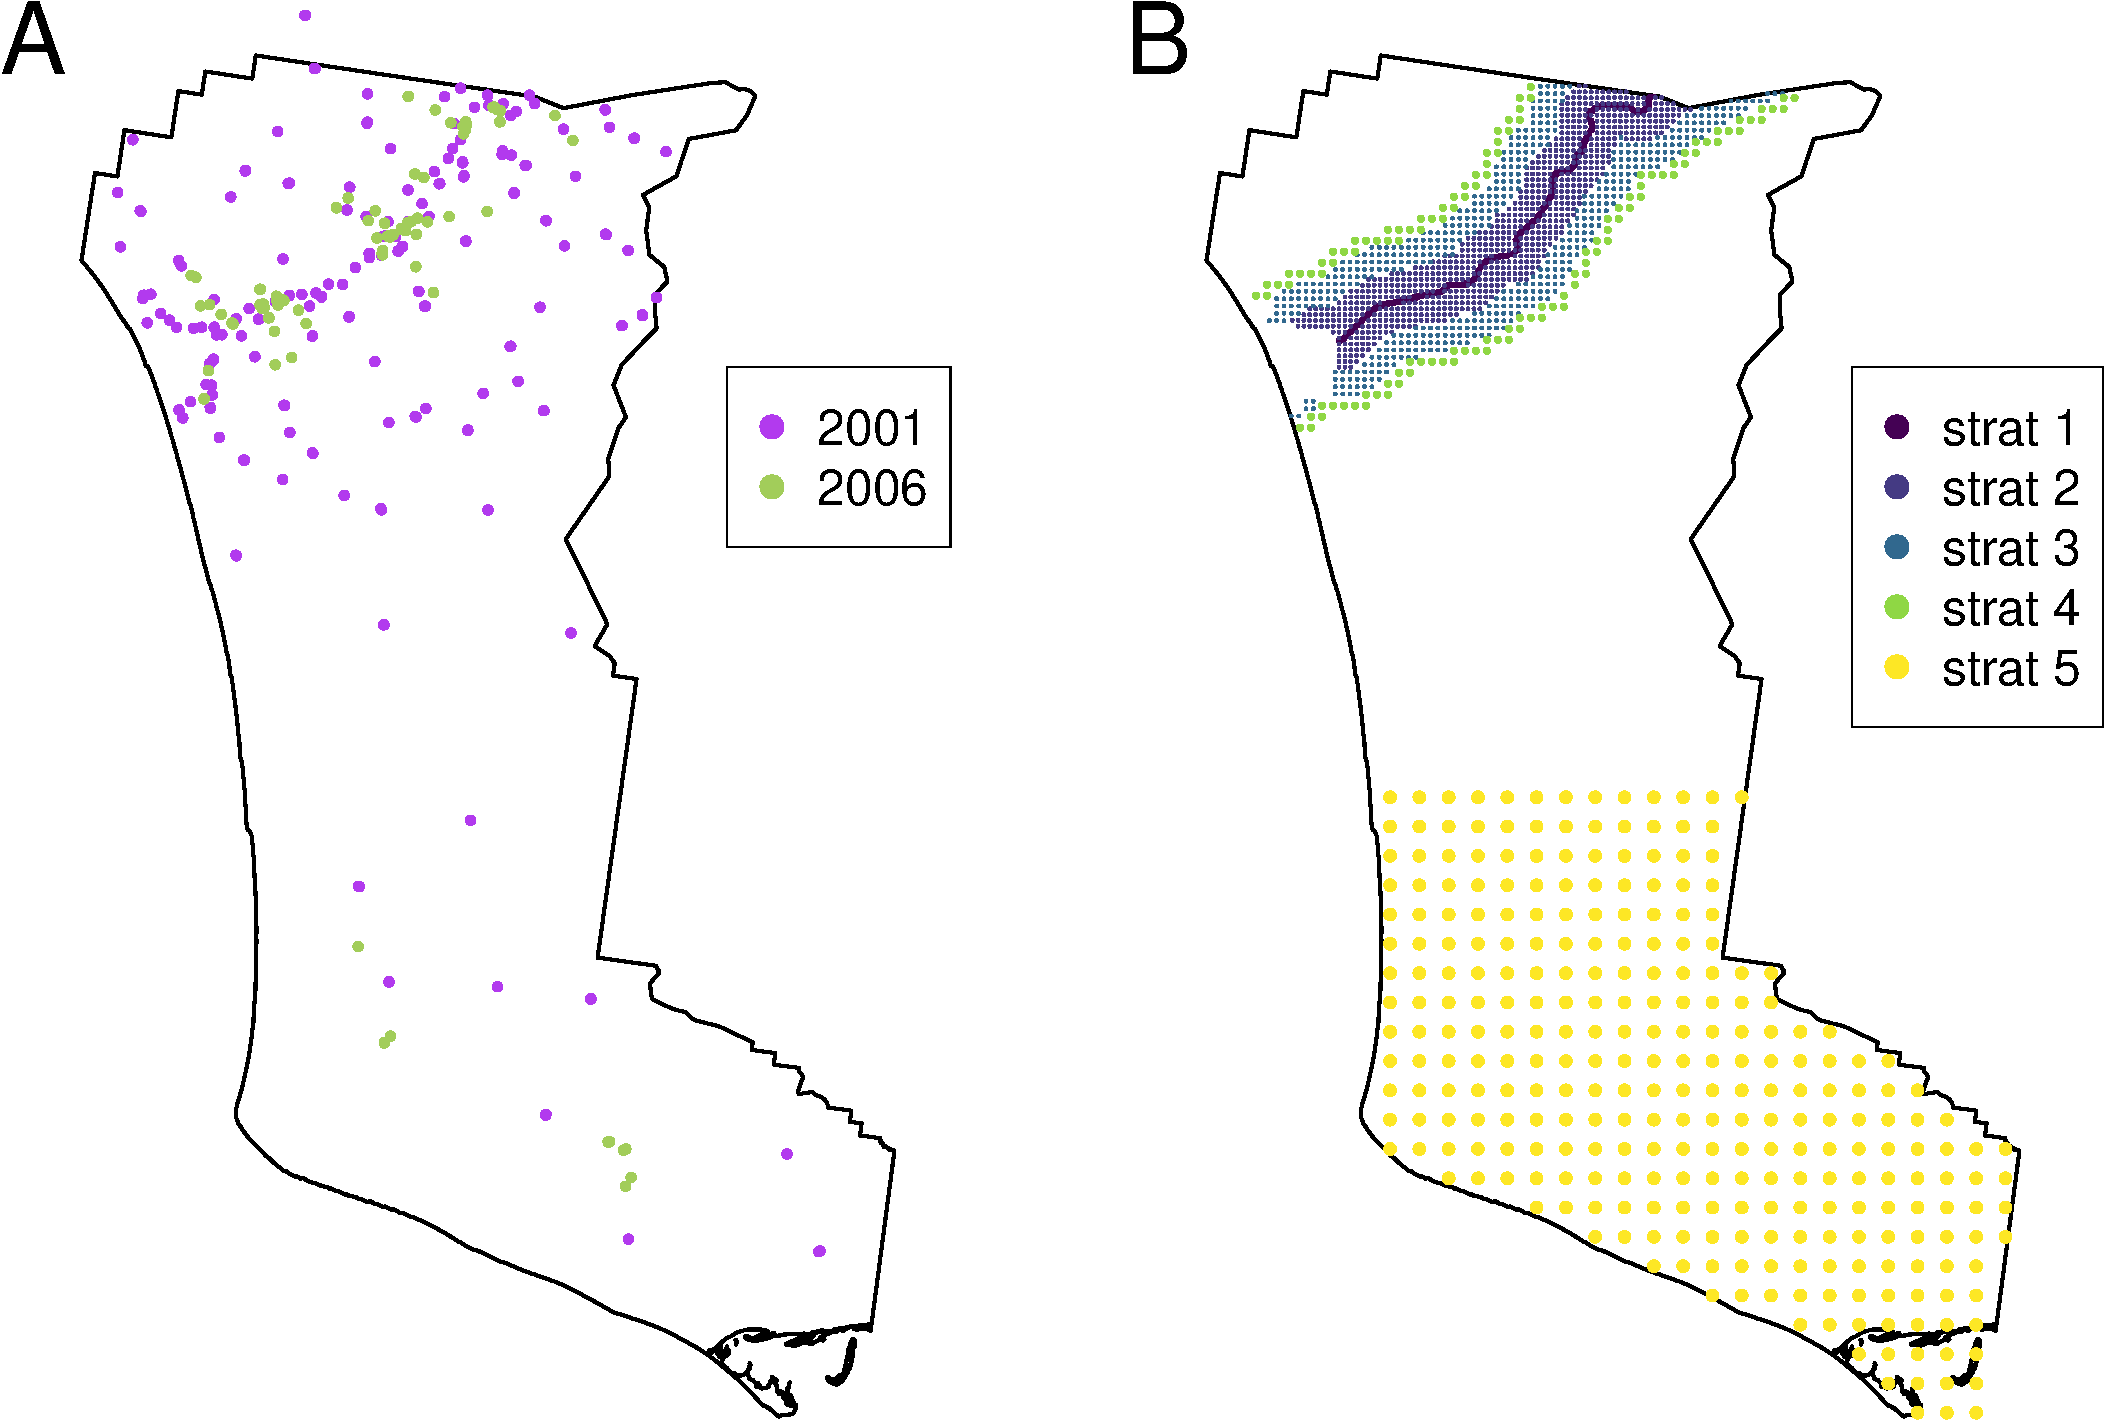
\includegraphics[width=0.6\textwidth]{Chapter1/figure/RedDog_sampling.pdf}
\caption{A. Map showing sample locations for two years in and around Cape Krusenstern National Park. B. Prediction locations at various densities, with higher densities near the road (Strata 1). \label{fig:RedDogSampling}}
\end{center}
\end{figure}

\begin{figure}
\begin{center}
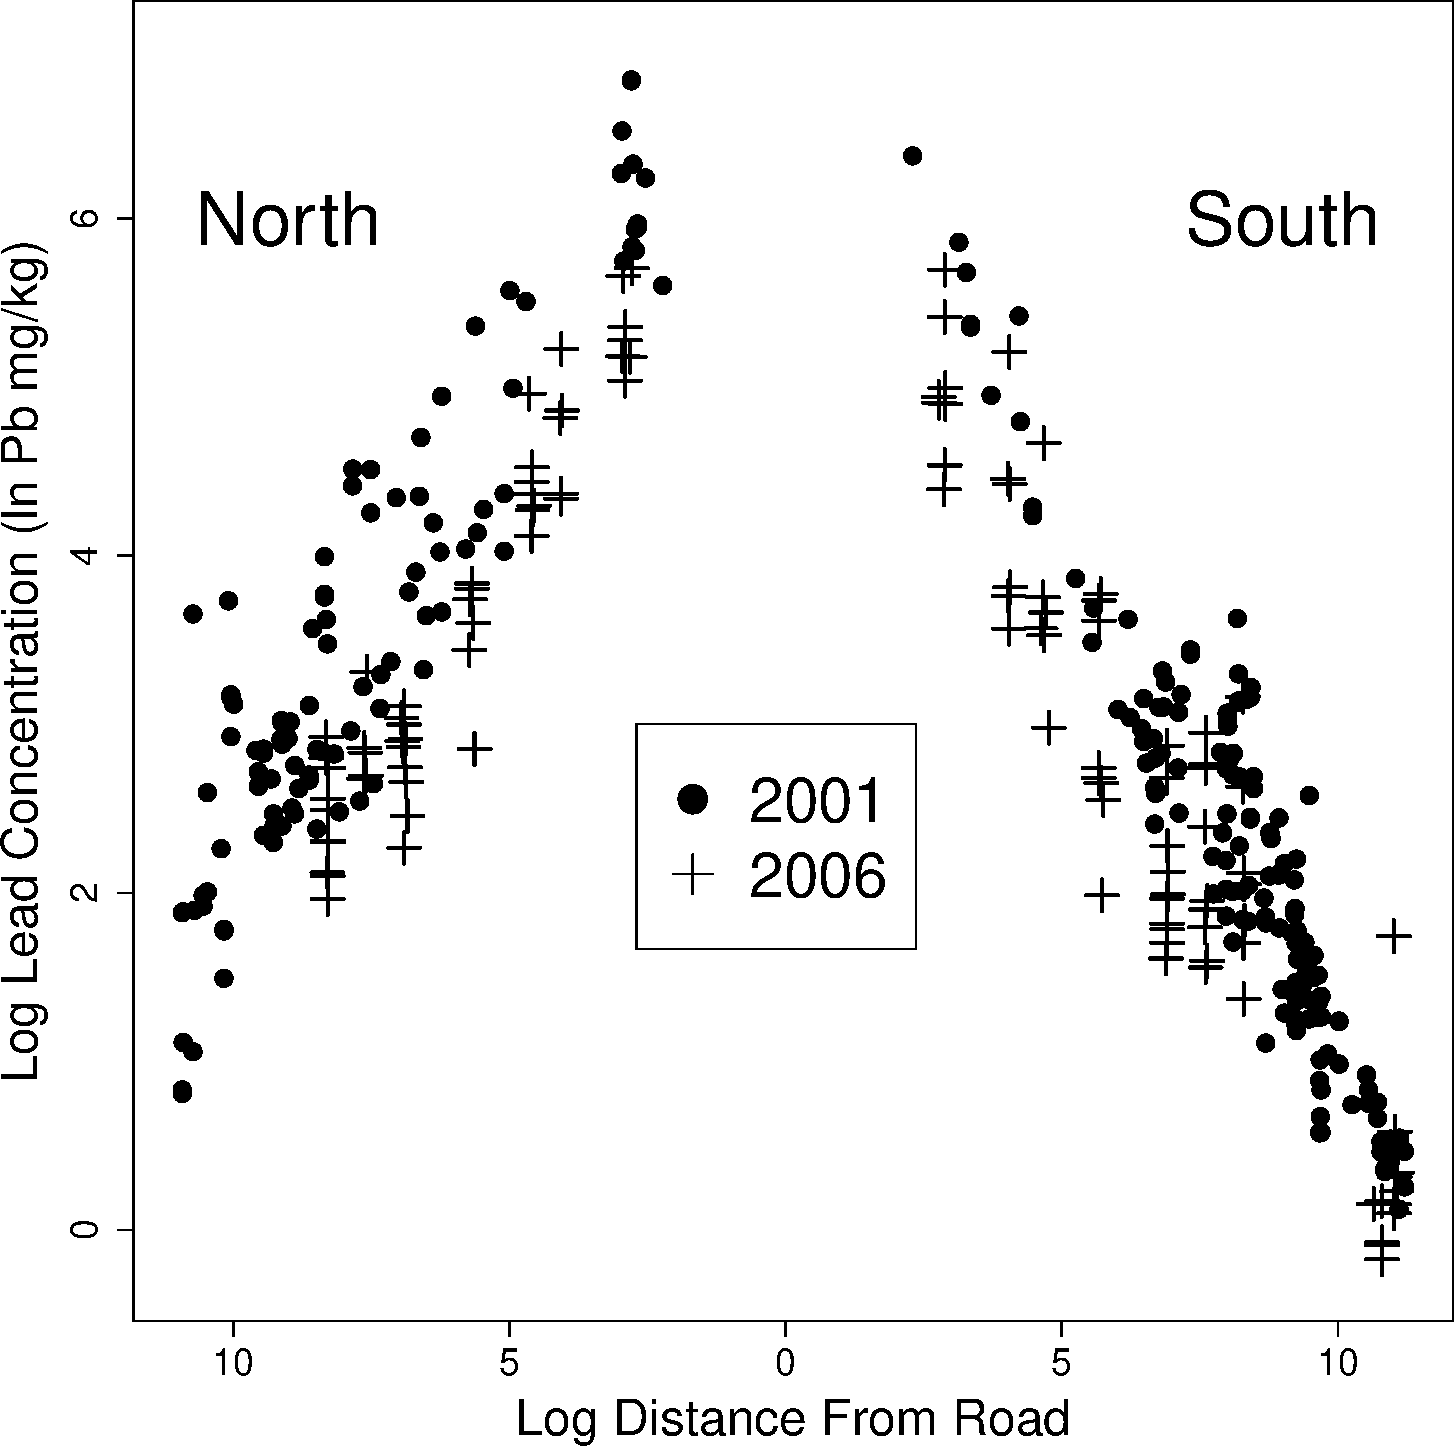
\includegraphics[width=0.6\textwidth]{Chapter1/figure/RedDog_DistRoad.pdf}
\caption{Log concentrations of zinc in moss tissues as a function of both the side of the road (negative numbers are north, while positive numbers are south) and the log of the distance from the road.  Data from both years 2001 and 2006 are shown.\label{fig:RedDogDistRoad}}
\end{center}
\end{figure}

Some questions that might be posed for these data include:
\begin{itemize}
\item Is there a significant relationship between zinc concentration and distance from road?
\item Is there a significant difference in the relationship between zinc concentration and distance from road on the north side of the road versus the south side?
\item In response to the analysis of the 2001 data, trucks on the haul road began using hydraulic covers rather than tarps to minimize dust escaping while hauling the ore.  Is there a significant difference in the relationship between zinc concentration and distance from road in 2006 versus 2001 -- i.e., did the hydraulic covers help?
\item After accounting for the covariates, is there still spatial dependence in the data, and if so, must we account for it?  That is, how does residual spatial autocorrelation affect our estimates of the relationships that we explored in the previous questions?
\item Can we combine covariates and spatial autocorrelation to predict zinc concentrations  at arbitrary unsampled locations, or obtain averaged values over selected subregions (given by the strata in Figure \ref{fig:RedDogSampling}B)?
\end{itemize}

$\quad\blacksquare$
\vspace{.5in}
%------------------------------------------------------------------------------
%          End of Examples
%------------------------------------------------------------------------------


As can be seen from these examples, the specific questions associated with particular spatial datasets may vary.  However, some general types of inquiries are common to many applications.  For example, frequently one wants to understand how the spatial variable $y$ varies over the spatial domain.  Both large-scale variability (``spatial trend") and small-scale variability (``spatial dependence" or ``residual spatial autocorrelation") are of interest.  Also, it is often the case that one wants to predict the value of $y$, or perhaps the value of $y$ minus the error made in its observation, at a set of {\em prediction sites} ${\cal P}\subset{\cal A}$.  This problem is called {\em spatial prediction}, and the quantities to be predicted are called {\em spatial predictands}.  Prediction sites, like data sites, may be either subregions or points, and they may be a subset or superset of the data sites or completely distinct from them.  Furthermore, prediction sites need not have the same support as data sites, leading to what is sometimes called a change-of-support problem; for example, in a geostatistical setting where all the data sites are (idealized as) points, one may wish to predict the average of the response over a relatively large subregion.  If ${\cal P}$ is either a finite partition of ${\cal A}$ or the set of all points in ${\cal A}$, then spatial prediction essentially amounts to producing a map of predictions over ${\cal A}$.  In practice, it suffices to consider a (possibly very long) vector of predictands, which we denote throughout as ${\bf u}=(U(S_{n+1}),U(S_{n+2}),\ldots,U(S_{n+K}))^T$, where $K$ is the number of prediction sites, $S_{n+k}$ is the $k$th prediction site, and $U(S_{n+k})$ is the predictand at that site.

%%%%%%%%%%%%%%%%%%%%%%%%%%%%%%%%%%%%%%%%%%%%%%%%%%%%%%%%%%%%%%%%%%%%%%%%%%%%%%%%%%
%%%%%%%%%%%%%%%%%%%%%%%%%%%%%%%%%%%%%%%%%%%%%%%%%%%%%%%%%%%%%%%%%%%%%%%%%%%%%%%%%%
%                Section: Sampling Framework
%%%%%%%%%%%%%%%%%%%%%%%%%%%%%%%%%%%%%%%%%%%%%%%%%%%%%%%%%%%%%%%%%%%%%%%%%%%%%%%%%%
%%%%%%%%%%%%%%%%%%%%%%%%%%%%%%%%%%%%%%%%%%%%%%%%%%%%%%%%%%%%%%%%%%%%%%%%%%%%%%%%%%

\section{Sampling Framework}

In order to make statistical inferences about spatial trend and spatial dependence, a probabilistic model for the data must be specified.  Accordingly, we suppose that the responses $y_1,\ldots, y_n$ are the observed values of random variables $Y_1=Y(S_1),\ldots,Y_n=Y(S_n)$, and later in this chapter we will introduce a class of models for these variables called {\em spatial linear models}.  Here, we merely focus on a sampling framework that is appropriate for these random variables.

The classical random sampling framework, with its assumptions that the random variables are independent and identically distributed, is generally too restrictive in this setting.  Spatial data often adhere, to a large extent, to Tobler's first law of geography, which says that ``everything is related to everything else, but near things are more related than distant things" \citep{tobler1970computer}.  In particular, spatial data generally are not identically distributed but instead vary across their domain in a manner that appears to include a smooth (but nonconstant) systematic component --- a spatial trend.  Furthermore, because some spatial processes and interactions may operate at relatively small scales, residuals from the trend corresponding to sites close to one another tend to be more similar than residuals corresponding to sites further apart --- spatial dependence.  Thus, the responses are not properly regarded as independent observations from a univariate distribution, but rather as comprising a single, vector-valued observation ${\bf y}=(y_1,y_2,\ldots,y_n)^T$ from an $n$-variate distribution, and any probabilistic model for ${\bf y}$ should allow for spatial trend and spatial dependence.

For some purposes, it may be useful to imagine the set of observed responses as a subset of a larger set of observed and ``potential" responses.  In the areal case, for example, for one reason or another the response may not be observed at every subregion of the partition of ${\cal A}$ and it may be desirable to predict the responses corresponding to those subregions where it was not observed.  Alternatively, one may wish to predict the response corresponding to a subregion that lies within one, or overlaps with two or more, of the $A_i$'s.  Regarding the observed response vector ${\bf y}$ as a subvector of a larger vector formed by appending the desired predictands to ${\bf y}$ may be convenient for solving these prediction problems.  In the geostatistical case, a potential response exists, in theory, at every point in ${\cal A}$, and for prediction of one or more of them it is useful to regard ${\bf y}$ as the finite, observed portion of an infinite collection of observed and potential responses $\{Y({\bf s}): {\bf s}\in{\cal A}\}$.

To perform spatial prediction statistically, we must regard the predictands, like the responses, as random variables.  The same considerations that led us to regard the responses as comprising a single realization from a multivariate distribution lead us to assume that the predictands likewise are not independent and identically distributed but have a multivariate distribution exhibiting spatial trend and spatial dependence.  Furthermore, because the predictands lie in the same spatial domain as the responses, the spatial trend of, and spatial dependence among, the predictands is likely to be related to that of the responses.  This suggests that we specify a probabilistic model for the joint distribution of ${\bf y}$ and ${\bf u}$ rather than for each separately.  In fact, in the geostatistical context, where the number of potential predictands is infinite, it may be convenient to specify a probabilistic model for the infinite collection of random variables $\{Y({\bf s}): {\bf s}\in{\cal A}\}$, henceforth referred to as a {\em geostatistical process}, or more generally for ${\bf y}$ and another random process $\{U({\bf s}): {\bf s}\in {\cal A}\}$ of predictands.

For some purposes, e.g.\ mere point estimation of spatial trend parameters under simple models, specifying a particular probability distribution for the (continuous) random variables representing the responses and predictands is unnecessary.  For inference that includes assigning measures of uncertainty to estimates or conclusions, however, distributional assumptions are necessary.  Accordingly, we invariably assume that the joint distribution of ${\bf y}$ and ${\bf u}$, possibly after a transformation, is multivariate normal (or nearly so).  In the geostatistical case, we will likewise assume that $\{Y({\bf s}): {\bf s}\in{\cal A}\}$ and/or any other relevant process of predictands is a {\em Gaussian process} (an infinite collection of random variables whose finite-dimensional distributions are all multivariate normal).  

Although we regard the responses and predictands as (normal) random variables, we take the covariates ${\bf z}_1,\ldots,{\bf z}_n$ to be nonrandom.  Arguably, in some applications it may be just as reasonable to regard one or more of the covariates as random as it is to so regard the response.  In such a situation the model must be interpreted as a model for the conditional distribution of ${\bf y}$ and the predictands, given the observed values of the covariates, and all inferences made on the basis of the model must be regarded as conditional (on the observed values of the covariates) rather than unconditional.  Furthermore, we assume that the sites (the $S_i$'s) are selected independently of ${\bf y}$.  That is, they are not {\em preferentially sampled}, using the terminology of \citet{diggle2010geostatistical}.

%%%%%%%%%%%%%%%%%%%%%%%%%%%%%%%%%%%%%%%%%%%%%%%%%%%%%%%%%%%%%%%%%%%%%%%%%%%%%%%%%%
%%%%%%%%%%%%%%%%%%%%%%%%%%%%%%%%%%%%%%%%%%%%%%%%%%%%%%%%%%%%%%%%%%%%%%%%%%%%%%%%%%
%      Section: Mean Functions, Covariance Functions, and Semivariograms
%%%%%%%%%%%%%%%%%%%%%%%%%%%%%%%%%%%%%%%%%%%%%%%%%%%%%%%%%%%%%%%%%%%%%%%%%%%%%%%%%%
%%%%%%%%%%%%%%%%%%%%%%%%%%%%%%%%%%%%%%%%%%%%%%%%%%%%%%%%%%%%%%%%%%%%%%%%%%%%%%%%%%

\section{Mean Functions, Covariance Functions, and Semivariograms}
So far, the notions of spatial trend and spatial dependence have been rather loosely defined.  For the class of spatial linear models, these spatial data features correspond to well-defined functions known as the mean function, covariance function, and semivariogram.  This section presents some background on these, beginning with a review of moments of one or two random variables. 

%------------------------------------------------------------------------------
%          Subsection: Moments of one or two random variables
%------------------------------------------------------------------------------
\subsection{Moments of one or two random variables}
Suppose that $Y$ is a discrete random variable with probability mass function $f(y)$, where $f(y)>0$ for $y\in{\cal Y}$.  If the sum
\begin{equation}\label{Ediscrete}
\sum_{y\in{\cal Y}}u(y)f(y)
\end{equation}
exists, then it (the sum) is called the {\bf expectation} of $u(Y)$.  Suppose, on the other hand, that
$Y$ is an (absolutely) continuous random variable with probability density function $f(y)$, where $f(y)>0$ for $y\in{\cal Y}$.  If
\begin{equation}\label{Econtinuous}
\int_{\cal Y}u(y)f(y)\,dy
\end{equation}
exists, then it (the integral) is called the {\bf expectation} of $u(Y)$.  A more general definition of expectation can be given for any type of random variable, but for our purposes the definitions above will suffice.  In any case, the expectation of $u(Y)$ is written as $E(u(Y))$.

Two very important types of expectations are the moments and central moments of order $k$ ($k=1,2,\ldots)$, corresponding to setting $u(Y)=Y^k$ and $u(Y)=(Y-E(Y))^k$, respectively, in either (\ref{Ediscrete}) or (\ref{Econtinuous}) (depending on whether $Y$ is discrete or continuous).  When they exist, the first-order moment $E(Y)$ and the second-order central moment $E[(Y-E(Y))^2]$ are called the mean and the variance, respectively.  Conventionally, the mean of $Y$ is often represented by the Greek symbol $\mu$, and the variance of $Y$ is often represented by $\sigma^2$.  We shall follow these conventions throughout, using subscripts or other devices as necessary to distinguish means and variances for different random variables (such as those corresponding to different spatial locations) from one another.  The variance of $Y$ may also be written as Var$(Y)$.  

It follows easily from the definition of expectation that
\begin{equation}\label{expectationrule}
E(c_1u_1(Y)+c_2u_2(Y))=c_1E(u_1(Y))+c_2E(u_2(Y))
\end{equation}
where $c_1$ and $c_2$ are nonrandom real numbers and $u_1(\cdot)$ and $u_2(\cdot)$ are functions whose expectations exist.  Using (\ref{expectationrule}), many important facts about means and variances can be obtained.  For example, a well-known alternative formula for the variance of $Y$ may be obtained via the following calculation:
\begin{equation}\label{altvariance}
\mbox{Var}(Y)=E[(Y-\mu)^2]=E[Y^2-2\mu Y+\mu^2]=E(Y^2)-\mu^2.
\end{equation}
Two other important facts derived as special cases of (\ref{expectationrule}) are
\begin{equation}\label{Elinearform}
E(aY+b)=a\mu+b
\end{equation}
and
\begin{equation}\label{Varlinearform}
\mbox{Var}(aY+b)=a^2\sigma^2.
\end{equation}

Now suppose that $Y_1$ and $Y_2$ are two random variables, either both discrete or both continuous, with joint probability mass function or density function $f(y_1,y_2)$ on support ${\cal Y}$.  Then the expectation of $u(Y_1,Y_2)$, when it exists, is defined by a straightforward extension of the definition given earlier.  In the discrete case,
\[ E(u(Y_1,Y_2))=\sum_{(y_1,y_2)\in{\cal Y}}u(y_1,y_2)f(y_1,y_2), \]
and in the continuous case,
\[ E(u(Y_1,Y_2))=\iint\limits_{\cal Y}u(y_1,y_2)f(y_1,y_2)\,dy_1\,dy_2. \]
From the definition, it follows that
\begin{equation}\label{expectationrulebivariate}
E(c_1u_1(Y_1,Y_2)+c_2u_2(Y_1,Y_2))=c_1E(u_1(Y_1,Y_2))+c_2E(u_2(Y_1,Y_2)).
\end{equation}

It turns out that the means $\mu_1$ and $\mu_2$, and variances $\sigma_1^2$ and $\sigma_2^2$, of $Y_1$ and $Y_2$ (when they exist) may be obtained using either the bivariate expectation just described [with $u(Y_1,Y_2)=Y_i$ for $\mu_i$ and $u(Y_1,Y_2)=(Y_i-E(Y_i))^2$ for $\sigma_i^2$, for $i=1$ or 2] or the previous univariate expectation [with the marginal distributions of $Y_1$ and $Y_2$ playing the role previously played by $f(y)$].  However, there are other important expectations in spatial statistics that require the bivariate approach.  One of these is the covariance.  The {\bf covariance} of (or between) $Y_1$ and $Y_2$, when it exists, is defined as
\[ \mbox{Cov}(Y_1,Y_2)=\mbox{E}[(Y_1-\mu_1)(Y_2-\mu_2)]\equiv\sigma_{12}. \]
The covariance of $Y_1$ and $Y_2$ exists if and only if $\sigma_1^2$ and $\sigma_2^2$ exist (as a consequence of the Cauchy-Schwartz inequality).  Observe that Cov($Y_1,Y_1)=\mbox{Var}(Y_1)$ and Cov($Y_2,Y_1)=\mbox{Cov}(Y_1,Y_2)$, so symbols $\sigma_1^2$ and $\sigma_{11}$ can be used interchangeably, as can $\sigma_{12}$ and $\sigma_{21}$.  Using (\ref{expectationrulebivariate}), the following additional facts can be obtained:
\begin{eqnarray}
\mbox{Cov}(Y_1,Y_2) & = & E(Y_1Y_2)-\mu_1\mu_2, \label{covfact1} \\
\mbox{Cov}(a_1Y_1+b_1,a_2Y_2+b_2) & = & a_1a_2\sigma_{12}, \label{covfact2} \\
\mbox{Var}(a_1Y_1+a_2Y_2) & = & a_1^2\sigma_1^2+a_2^2\sigma_2^2+2a_1a_2\sigma_{12}. \label{covfact3}
\end{eqnarray}
In the special case $Y_1=Y_2$, (\ref{covfact1}) reduces to (\ref{altvariance}); if, in addition $a_1=a_2$ and $b_1=b_2$, then (\ref{covfact2}) reduces to (\ref{Varlinearform}).

As its name suggests, the covariance of $Y_1$ and $Y_2$ measures, in a certain sense, the extent to which $Y_1$ and $Y_2$ co-vary or, in other words, how they ``depend" on each other.  However, there are two limitations to this interpretation.  First, the magnitude of $\sigma_{12}$ depends on the scale of measurement, so by itself it cannot be regarded as a measure of dependence.  A unitless version of the covariance is the {\bf correlation}, written as Corr($Y_1,Y_2)$ and defined as
\[ \mbox{Corr}(Y_1,Y_2)=\frac{\mbox{Cov}(Y_1,Y_2)}{\sqrt{\mbox{Var}(Y_1)\mbox{Var}(Y_2)}}=\frac{\sigma_{12}}{\sqrt{\sigma_1^2\sigma_2^2}}\equiv\rho_{12}, \]
provided that $\sigma_1^2$ and $\sigma_2^2$ are positive.  Observe that Corr($Y_1,Y_1)=1$.  It can be shown that $-1\leq\rho_{12}\leq 1$ (as another consequence of the Cauchy-Schwartz inequality), so the correlation solves the scaling issue.  The second limitation is that $\rho_{12}$ measures the strength of only the {\em linear} dependence between $Y_1$ and $Y_2$.  That is, if $Y_1$ and $Y_2$ are independent, then $\rho_{12}=0$; but the converse is not generally true.  For example, if $Y_1=Y_2^2$, then $\rho_{12}=0$ despite the perfect but nonlinear dependence between $Y_1$ and $Y_2$.  Thus the correlation generally is an imperfect measure of the dependence between two variables, but it is still quite useful.  In the special case in which $Y_1$ and $Y_2$ have a bivariate normal distribution, zero correlation {\em does} imply independence.

Another bivariate moment used frequently in spatial statistics, but rarely introduced in mathematical statistics courses, is the {\bf semivariance}.  The semivariance of $Y_1$ and $Y_2$ is defined as
\[ \gamma_{12}=\frac{1}{2}\mbox{Var}(Y_1-Y_2) \]
provided that this variance exists.  Observe that $\gamma_{12}=\gamma_{21}$, 
\begin{equation}\label{semivariance0}
\gamma_{11}=0,
\end{equation}
and
\begin{equation}\label{altsemivariance}
\gamma_{12} = \frac{1}{2}\mbox{E}[(Y_1-Y_2)^2]\quad\mbox{if $E(Y_1-Y_2)=0$.}
\end{equation}
Using (\ref{covfact3}), it is easy to show that
\begin{equation}\label{semivariancefact1}
\gamma_{12} = \frac{1}{2}(\sigma_1^2+\sigma_2^2-2\sigma_{12})\quad\mbox{if $\sigma_1^2$ and $\sigma_2^2$ exist}, 
\end{equation}
and
\begin{equation}\label{semivariancefact2}
\gamma_{12} = \sigma^2-\sigma_{12}=\sigma^2(1-\rho_{12})\quad\mbox{if $\sigma_1^2=\sigma_2^2\equiv\sigma^2$}.
\end{equation}
By (\ref{semivariancefact1}), the semivariance of two variables exists if their variances exist.  The converse is not generally true, however.  To see this, let $Y_1=X_1+W$ and $Y_2=X_2+W$, where $X_1$ and $X_2$ are random variables with finite variances but $W$ is a random variable, independent of $X_1$ and $X_2$, whose variance does not exist (e.g., a Cauchy random variable).  Then neither Var($Y_1$) nor Var($Y_2$) exist, but $\frac{1}{2}$Var($Y_1-Y_2)=\frac{1}{2}\mbox{Var}(X_1-X_2)$, which exists by (\ref{semivariancefact1}).

%------------------------------------------------------------------------------
%    Subsection: First-order and second-order moments of a random vector
%------------------------------------------------------------------------------

\subsection{First-order and second-order moments of a random vector}

The definitions of moments may be extended from one- and two-variable settings to situations with any finite number $n$ of random variables $Y_1,\ldots,Y_n$, i.e., to a random $n$-vector ${\bf y}$.  We skip a formal definition of expectation in this setting and instead immediately give extensions of some of the facts we provided earlier for the bivariate case.  If $Y_1,\ldots,Y_n$ are random variables whose variances $\sigma_1^2,\ldots,\sigma_n^2$ exist, and $\mu_1,\ldots,\mu_n$ represent their means and $\sigma_{ij}$ $(i\neq j=1,\ldots,n)$ represent their covariances, then the following rules hold for the mean, variance, and covariance of arbitrary linear combinations of the variables:
\begin{eqnarray}
\mbox{E}\left(\sum_{i=1}^na_iY_i\right) & = & \sum_{i=1}^na_i\mu_i, \label{vectormoment1} \\
\mbox{Var}\left(\sum_{i=1}^na_iY_i\right) & = & \sum_{i=1}^na_i^2\sigma_i^2+2\sum_{i=1}^n\sum_{j=i+1}^na_ia_j\sigma_{ij} \label{vectormoment2} \\
& = & \sum_{i=1}^na_i^2\sigma_i^2+2\sum_{i=1}^n\sum_{j=i+1}^na_ia_j\sigma_{i}\sigma_j\rho_{ij}, \label{vectormoment3} \\
\mbox{Cov}\left(\sum_{i=1}^na_iY_i,\sum_{j=1}^nb_jY_j\right) & = & \sum_{i=1}^n\sum_{j=1}^na_ib_j\sigma_{ij} \label{vectormoment4} \\
& = & \sum_{i=1}^n\sum_{j=1}^na_ib_j\sigma_i\sigma_j\rho_{ij}. \label{vectormoment5}
\end{eqnarray}

For economy of expression, it can be helpful to organize all of the means in a $n$-dimensional vector $\bmu$, called the {\bf mean vector} of ${\bf y}$:
\[ \bmu=\left(\begin{array}{c}\mu_1\\\mu_2\\ \vdots \\ \mu_n\end{array}\right). \]
Likewise, it is helpful to organize all the variances and covariances in an $n\times n$ matrix $\bSigma$:
\[ \bSigma=\left(\begin{array}{cccc}
\sigma_1^2 & \sigma_{12} & \cdots & \sigma_{1n} \\
\sigma_{21} & \sigma_2^2 & \cdots & \sigma_{2n} \\
\vdots & \vdots & & \vdots \\
\sigma_{n1} & \sigma_{n2} & \cdots & \sigma_n^2 \end{array}\right) . \] 
Provided that $\sigma_i^2>0$ for all $i$, we can similarly construct an $n\times n$ matrix of correlations $\brho$:
\[ \brho=\left(\begin{array}{cccc}
1 & \rho_{12} & \cdots & \rho_{1n} \\
\rho_{21} & 1 & \cdots & \rho_{2n} \\
\vdots & \vdots & & \vdots \\
\rho_{n1} & \rho_{n2} & \cdots & 1 \end{array}\right). \]
$\bSigma$ is called the {\bf variance-covariance matrix}, or simply the {\bf covariance matrix}, of ${\bf y}$, and $\brho$ is called the {\bf correlation matrix} of ${\bf y}$.  The two matrices are related via the equation
\[ \brho=\mbox{diag}\left(\frac{1}{\sqrt{\sigma_{11}}},\ldots,\frac{1}{\sqrt{\sigma_{nn}}}\right)\bSigma\,\mbox{diag}\left(\frac{1}{\sqrt{\sigma_{11}}},\ldots,\frac{1}{\sqrt{\sigma_{nn}}}\right) \]
where for any $n$-vector ${\bf a}$, diag$({\bf a})$ is defined as the $n\times n$ matrix with its main diagonal elements given by the elements of ${\bf a}$ and all of its off-diagonal elements equal to zero.  Finally, we may define the $n\times n$ {\bf semivariance matrix}
\[ \bGamma=\left(\begin{array}{cccc}
0 & \gamma_{12} & \cdots & \gamma_{1n} \\
\gamma_{21} & 0 & \cdots & \gamma_{2n} \\
\vdots & \vdots & & \vdots \\
\gamma_{n1} & \gamma_{n2} & \cdots & 0 \end{array}\right) . \]
All of the main diagonal elements of $\bGamma$ are equal to 0 by the extension of (\ref{semivariance0}) to $n$ variables.

Using the matrices just defined, equations (\ref{vectormoment1}), (\ref{vectormoment2}), and (\ref{vectormoment4}) may be re-expressed as follows:
\begin{eqnarray}
E({\bf a}^T{\bf y}) & = & {\bf a}^T\bmu, \label{vm1reexpress} \\
\mbox{Var}({\bf a}^T{\bf y}) & = & {\bf a}^T\bSigma{\bf a}, \label{vm2reexpress} \\
\mbox{Cov}({\bf a}^T{\bf y},{\bf b}^T{\bf y}) & = & {\bf a}^T\bSigma{\bf b}. \label{vm4reexpress}
\end{eqnarray}

The matrices of moments defined above satisfy several important properties.  First, because $\sigma_{ij}=\sigma_{ji}$ and $\gamma_{ij}=\gamma_{ji}$ for all $i$ and $j$, the covariance, correlation, and semivariance matrices are symmetric.  Second, as a straightforward consequence of (\ref{vm2reexpress}), the covariance and correlation matrices are {\em nonnegative definite}.  (Recall that an $n\times n$ matrix ${\bf A}$ is said to be nonnegative definite if ${\bf x}^T{\bf Ax}\geq 0$ for all $n$-vectors ${\bf x}$.)  Last, the semivariance matrix is {\em conditionally nonpositive definite}, meaning that
\begin{equation}\label{condnonposdef}
{\bf x}^T\bGamma{\bf x}\leq 0 \quad\mbox{for all $n$-vectors ${\bf x}$ satisfying ${\bf x}^T{\bf 1}=0$}.
\end{equation}
Verifying this last property is left as an exercise.

%------------------------------------------------------------------------------
%  Subsection: First-order and second-order moments of a geostatistical process
%------------------------------------------------------------------------------

\subsection{First-order and second-order moments of a geostatistical process}
The vectors and matrices of moments described in the previous subsection are sufficient for models for a random vector such as ${\bf y}$ or ${\bf u}$, but they are insufficient when modeling a geostatistical process.  For the latter, there is a mean and a variance corresponding to the variable at each of uncountably many points, and a covariance, correlation, and semivariance corresponding to the variables at uncountably many pairs of points (assuming that these moments exist).  It is natural, then, to represent the mean, variance, covariance (or correlation), and semivariance of a geostatistical process as functions of those points.  In particular, the {\bf mean function} and {\bf covariance function} of $\{Y({\bf s}):{\bf s}\in{\cal A}\}$ may be defined as
\[ \mu({\bf s})=E(Y({\bf s})), \quad {\bf s}\in{\cal A} \]
and
\[ \sigma({\bf s},{\bf s}')=\mbox{Cov}(Y({\bf s}),Y({\bf s}')),\quad {\bf s},{\bf s}'\in{\cal A}, \]
respectively.  The covariance function provides not only the covariance between the random variables at any distinct locations ${\bf s}$ and ${\bf s}'$, but also the variance at any location ${\bf s}$ (by substituting ${\bf s}$ for ${\bf s}'$ in the function).
Along the same lines, the {\bf correlation function} and {\bf semivariogram} are defined as
\[ \rho({\bf s},{\bf s}')=\mbox{Corr}(Y({\bf s}),Y({\bf s}')), \quad {\bf s},{\bf s}'\in{\cal A} \]
and
\[ \gamma({\bf s},{\bf s}')=\frac{1}{2}\mbox{Var}(Y({\bf s})-Y({\bf s}')),\quad {\bf s},{\bf s}'\in{\cal A}, \]
respectively.

It follows immediately from the definitions of the covariance function, correlation function, and semivariogram that they are {\em symmetric}, i.e., they satisfy $f({\bf s},{\bf s}')=f({\bf s}',{\bf s})$ (for $f=\sigma,\rho,\gamma$) for all ${\bf s},{\bf s}'\in{\cal A}$.  Furthermore, as a consequence of the nonnegative definiteness of the covariance matrix of a random vector noted in Section 1.3.2, the covariance function is {\em positive definite}, meaning that
\begin{equation}\label{defnpositivedefinitefn}
\sum_{i=1}^{n}\sum_{j=1}^{n}a_ia_j\sigma({\bf s}_i,{\bf s}_j)\geq 0\quad\mbox{for all $n$, all real numbers $a_1,\ldots,a_n$, and all points ${\bf s}_1,\ldots,{\bf s}_n.$}
\end{equation}
The correlation function likewise is positive definite.  And, as a consequence of the conditional nonpositive definiteness of the semivariance matrix of a random vector noted in Section 1.3.2, the semivariogram is {\em conditionally negative definite}, meaning that
\begin{equation}\label{defncondnegativedefinitefn}
\sum_{i=1}^{n}\sum_{j=1}^{n}a_{i}a_{j}\gamma({\bf s}_{i},{\bf s}_{j})
\leq 0 \quad\mbox{for all $n$, all real numbers $a_{1}, 
\ldots, a_{n}$ such that $\sum_{i=1}^{n}a_{i}=0$, and all ${\bf s}_1,\ldots,{\bf s}_n$}.
\end{equation}

The reader may have noticed a difference in the terminology used to describe the properties of covariance and semivariance matrices on the one hand (nonnegative definite and conditionally nonpositive definite), and the analogous properties of the covariance function and semivariogram on the other (positive definite and conditionally negative definite).  This difference reflects a well established, though regrettable, tradition in the literature, from which we are loathe to depart.  

%------------------------------------------------------------------------------
%  Subsection: Spatially structured first-order and second-order moments
%------------------------------------------------------------------------------

\subsection{Spatially structured first-order and second-order moments}

In the classical statistics framework, the moments (when they exist) of a random variable (or random vector) can often be estimated effectively by the corresponding sample moments, or minor modifications thereof, of a sample drawn from the distribution of the random variable (or random vector).  For example, if
\[ \left(\begin{array}{c}Y_{11} \\ Y_{21} \end{array}\right),\left(\begin{array}{c}Y_{12} \\ Y_{22}\end{array}\right),\ldots,\left(\begin{array}{c}Y_{1n} \\ Y_{2n}\end{array}\right) \]
are a sample (of size $n$) drawn from a bivariate distribution, then one may estimate $\mu_i$ by $(1/n)\sum_{j=1}^{n}Y_{ij}$, $\sigma_i^2$ by $[(1/(n-1)]\sum_{j=1}^{n}(Y_{ij}-\bar{Y}_{i})^2$, and $\sigma_{12}$ by $[(1/(n-1)]\sum_{j=1}^{n}(Y_{1j}-\bar{Y}_{1})(Y_{2j}-\bar{Y}_2)$.  The success of this estimation approach rests on two features of classical statistical inference: low dimensionality of the random vector relative to the sample size $n$, and independence of the variables comprising the sample.  However, in the spatial context neither of these features generally is realistic: the dimension of the response vector is equal to $n$ and, as noted previously, the vector of observed responses represents only one observation from a multivariate distribution.  How can we possibly estimate moment functions from data that are so limited?  In general we cannot, but if enough additional structure is imposed on those functions, it may become possible to do so.

One type of structure that helps to make this possible is called {\em second-order stationarity}, which specifies that the mean is constant and that the covariance function depends on the spatial locations only through the displacement of one location from the other.  More formally, a geostatistical process on ${\cal A}$ with mean function $\mu({\bf s})$ and covariance function $\sigma({\bf s},{\bf s}')$ is said to be second-order stationary if $\mu({\bf s})=\mu$ (a common mean) for all ${\bf s}\in{\cal A}$ and
\begin{equation}\label{covstationary2}
\sigma({\bf s},{\bf s}') = \sigma({\bf s}-{\bf s}')\quad\mbox{for all ${\bf s},{\bf s}'\in{\cal A}$}.
\end{equation}
Whereas the covariance function generally is a function of $2d$ arguments (the elements of ${\bf s}$ and ${\bf s}'$), for a second-order stationary process the covariance function can be written in terms of only $d$ arguments, implying that the function can be represented as $\sigma({\bf h})$ where ${\bf h}$ is the $d$-dimensional vector of displacements in each of the coordinate directions.
Observe that second-order stationarity implies that $\sigma({\bf s},{\bf s})=\sigma({\bf 0})$, i.e., that the variance is constant over the spatial domain ${\cal A}$; this property, by itself, is sometimes called variance stationarity.  Second-order stationarity also implies that the correlation function likewise depends on the spatial locations only through their displacement, and that both the covariance and correlation functions are {\em even} functions (a function $f({\bf x})$ of $d$ variables is said to be even if $f(-{\bf x})=f({\bf x})$); this latter property follows from the symmetry of the more general functions noted in the previous subsection.

A somewhat weaker type of structure is known as {\em intrinsic stationarity}.  A geostatistical process on ${\cal A}$ with mean function $\mu({\bf s})$ and semivariogram $\gamma({\bf s},{\bf s}')$ is said to be intrinsically stationary if $\mu({\bf s})=\mu$ for all ${\bf s}\in{\cal A}$ and
\begin{equation}\label{intrinsicstationary2}
\gamma({\bf s},{\bf s}') = \gamma({\bf s}-{\bf s}')\quad\mbox{for all ${\bf s},{\bf s}'\in{\cal A}$}.
\end{equation}
To see that intrinsic stationarity is weaker than second-order stationarity, consider an arbitrary second-order stationary process with semivariogram $\gamma({\bf s},{\bf s}')$.  Because the variances of such a process exist and are all equal to a common value $\sigma^2$, we find, using (\ref{semivariancefact2}), that
\[ \gamma({\bf s},{\bf s}')=\sigma^2-\sigma({\bf s}-{\bf s}'), \]
which clearly depends on ${\bf s}$ and ${\bf s}'$ only through ${\bf h}={\bf s}-{\bf s}'$.  Thus, second-order stationarity implies intrinsic stationarity.  However, the converse is not true; a counterexample is provided in one of the exercises at the end of this chapter.

Stronger versions of second-order stationarity and intrinsic stationarity are obtained by requiring that the covariance function or semivariogram be not merely translation-invariant, but direction-invariant as well.  This structure is called {\em isotropy} (either second-order or intrinsic).  Thus, a second-order stationary process and its covariance function $\sigma({\bf s}-{\bf s}')$ are said to be isotropic if
\begin{equation}\label{isotropic1}
\sigma({\bf s}-{\bf s}') = \sigma(\|{\bf s}-{\bf s}'\|)\quad\mbox{for all ${\bf s},{\bf s}'\in{\cal A}$},
\end{equation}
and an intrinsically stationary process and its semivariogram $\gamma({\bf s}-{\bf s}')$ are said to be isotropic if
\begin{equation}\label{isotropic2}
\gamma({\bf s}-{\bf s}') = \gamma(\|{\bf s}-{\bf s}'\|)\quad\mbox{for all ${\bf s},{\bf s}'\in{\cal A}$}.
\end{equation}
Isotropic second-order stationarity implies further that $\rho({\bf s}-{\bf s}')=\rho(\|{\bf s}-{\bf s}'\|) \quad\mbox{for all ${\bf s},{\bf s}'\in{\cal A}$}$.  Under isotropy, the covariance and correlation functions and semivariogram may be written as a function of a single, scalar argument $r=\|{\bf s}-{\bf s}'\|$, representing the Euclidean distance between two points.  Furthermore, in the second-order stationary case, the {\em equicorrelation contours}, i.e., the locations of all the random variables of the process $Y(\cdot)$ that are equally correlated with any given variable $Y(\cdot)$, are the perimeters of circles (if $d=2$) or the surfaces of spheres (if $d=3)$ centered at the given variable's location.  A similar statement applies to the {\em equisemivariance contours} in the intrinsically stationary case.

If a geostatistical process is not isotropic, it is said to be {\em anisotropic}.  There are a variety of structured forms of anisotropy, the most useful of which is called {\em geometric anisotropy}. 
A second-order stationary process and its covariance function are said to be geometrically 
anisotropic if a positive definite matrix ${\bf B}$ exists such that
\[ \sigma({\bf s}-{\bf s}')=\sigma([({\bf s}-{\bf s}')^T{\bf B}({\bf s}-{\bf s}')]^{1/2}) \quad\mbox{for all ${\bf s},{\bf s}'\in{\cal A}$}. \]
A geometrically anisotropic intrinsically stationary process and semivariogram are defined analogously.
The equicorrelation (equisemivariance) contours of a geometrically anisotropic second-order (intrinsically) stationary process are the surfaces of $d$-dimensional ellipsoids.  Note that isotropy corresponds to the special case ${\bf B}={\bf I}$.

The types of stationarity introduced to this point impose restrictions only on the first- and second-order moments of a geostatistical process.  A stronger form, called {\em strict stationarity}, requires that the entire joint probability distribution of $\{Y({\bf s}): {\bf s}\in {\cal A}\}$, not merely its first- and second-order moments,
depends only on the relative positions of
sites.  That is, letting $F_{Y({\bf s}_1),\ldots,Y({\bf s}_n)}(x_1,\ldots,
x_n)$ denote the cumulative distribution function of $n$ variables $Y({\bf s}_1),\ldots,Y({\bf s}_n)$, it is required that
\[
F_{Y({\bf s}_1+{\bf h}),\ldots,Y({\bf s}_n+{\bf h})}(x_1,\ldots,
x_n) 
 = F_{Y({\bf s}_1),\ldots,Y({\bf s}_n)}(x_1,\ldots,
x_n) \] 
for all $n$, all locations ${\bf s}_1,\ldots,{\bf s}_n$, all displacements ${\bf h}$, and all 
$x_1,\ldots,x_n$.  This implies, for example, that Pr$[Y({\bf s}+{\bf h})\leq x]=$
Pr$[Y({\bf s})\leq x]$ for all ${\bf s}$, all ${\bf h}$, and all $x$; that is, that the marginal distributions of all the variables are identical.  It also implies that bivariate distributions are identical for any pairs of variables displaced by the same vector.

Thus, strict stationarity generally is stronger than second-order stationarity (which, as noted previously, is stronger than intrinsic stationarity).  However, in the case of a Gaussian geostatistical process, which is completely characterized by its mean and covariance functions, the two forms of stationarity coincide.  In other words, a second-order stationary Gaussian process is strictly stationary.  Therefore, for economy of expression we will refer to such a process as merely a {\em stationary Gaussian process}.

%%%%%%%%%%%%%%%%%%%%%%%%%%%%%%%%%%%%%%%%%%%%%%%%%%%%%%%%%%%%%%%%%%%%%%%%%%%%%%%%%%
%%%%%%%%%%%%%%%%%%%%%%%%%%%%%%%%%%%%%%%%%%%%%%%%%%%%%%%%%%%%%%%%%%%%%%%%%%%%%%%%%%
%      Section: Spatial Linear Models
%%%%%%%%%%%%%%%%%%%%%%%%%%%%%%%%%%%%%%%%%%%%%%%%%%%%%%%%%%%%%%%%%%%%%%%%%%%%%%%%%%
%%%%%%%%%%%%%%%%%%%%%%%%%%%%%%%%%%%%%%%%%%%%%%%%%%%%%%%%%%%%%%%%%%%%%%%%%%%%%%%%%%

\section{Spatial Linear Models}

Now we are ready to formally define the class of {\em spatial linear models} that is the subject of this book.  We begin by assuming that the responses $Y(S_1),\ldots,Y(S_n)$ forming the response vector ${\bf y}$ can be decomposed as follows:
\begin{equation}\label{spatiallinearmodel}
Y(S_i) = \mu(S_i,{\bf z}_i)+\epsilon(S_i).
\end{equation}
Here $\mu(S_i,{\bf z}_i)=E(Y(S_i))$ for all $i$, and $\epsilon(S_1),\ldots,\epsilon(S_n)$ are mean-zero, finite-variance, and possibly spatially correlated random variables representing residuals from the mean response at each site.  The mean of $Y(S_i)$ is thus assumed to be a function of the spatial coordinates and possibly other features of $S_i$ (e.g., its size in the areal case), and ${\bf z}_i$.  Similarly, the covariance of residuals at any two sites is assumed to be a function of the spatial coordinates and/or possibly other features of those sites (e.g., the length of their shared boundary), which is written as Cov$(\epsilon(S_i),\epsilon(S_j))=\sigma(S_i,S_j)\equiv\sigma_{ij}$.  It is further assumed that the mean is a {\em linear} function of a vector of $p$ unknown parameters $\bbeta=(\beta_1,\beta_2,\ldots,\beta_p)^T$, i.e., that 
\[ \mu(S_i,{\bf z}_i)={\bf x}_i^T\bbeta \]
where
\[ {\bf x}_i=\left(\begin{array}{c}{\bf f}(S_i) \\ {\bf z}_i\end{array}\right) \]
and ${\bf f}(S_i)$ is a vector-valued function of the coordinates and possibly other features of $S_i$.  This last assumption and the additivity of the residuals in (\ref{spatiallinearmodel}) are what define the model as a linear model.  The model may be written in conventional notation as
\begin{equation}\label{succinctslm}
{\bf y}={\bf X}\bbeta+\bepsilon
\end{equation}
by letting
\[ {\bf X}=\left(\begin{array}{c}{\bf x}_1^T \\ {\bf x}_2^T \\ \vdots \\ {\bf x}_n^T\end{array}\right)\quad\mbox{and}\quad\bepsilon=\left(\begin{array}{c}\epsilon(S_1)\\\epsilon(S_2)\\ \vdots \\ \epsilon(S_n)\end{array}\right), \]
where $E(\bepsilon)={\bf 0}$ and Var$({\bf y})=\mbox{Var}(\bepsilon)\equiv\bSigma=(\sigma_{ij})$.  The parameter space for $\bbeta$ is typically unconstrained, i.e., $\bbeta\in\mathbb{R}^p$.

If the elements of $\bSigma$ were known up to a multiplicative constant, the spatial linear model as defined to this point would be a special case of the so-called Aitken model, for which appropriate methods of analysis and inference may be found in many standard references on linear models.  In practice, however, the spatial data analyst often doesn't know precisely how the responses are correlated, but may be willing to assume that the spatial dependence is governed by a known, relatively parsimonious parametric covariance function which, when evaluated for every pair of data sites $(S_i,S_j)$, yields the elements of $\bSigma$.  Accordingly, in a spatial linear model it is assumed that the covariance between observed responses is a function of an $m$-vector $\btheta$, i.e., $\sigma_{ij}=\sigma(S_i,S_j;\btheta)$, which, like $\bbeta$, must be estimated from the data.  The joint parameter space for $\bbeta$ and $\btheta$ is generally taken to be
\begin{equation}\label{slmparameterspace}
\{(\bbeta,\btheta):\bbeta\in\mathbb{R}^p, \btheta\in\Theta\}
\end{equation}
where $\Theta$ is the set of $\btheta$ for which $\bSigma(\btheta)$ is positive definite.  The spatial linear model given by (\ref{succinctslm}), with moment assumptions $E(\bepsilon)={\bf 0}$ and Var$({\bf y})=\mbox{Var}(\bepsilon)\equiv\bSigma(\btheta)=(\sigma_{ij}(\btheta))$ and parameter space given by (\ref{slmparameterspace}), is then a special case of what is often called the general linear model.

Additional structure can be conferred to the model residuals $\epsilon(S_i)$ $(i=1,\ldots,n)$ by supposing that they may be decomposed as follows:
\begin{equation}\label{errordecomp}
\epsilon(S_i)=W(S_i)+\delta(S_i)
\end{equation}
where $W(S_1),\ldots,W(S_n)$ are zero-mean, finite-variance, and possibly spatially correlated random variables representing the ``noiseless" versions of $Y(S_1)-\mu(S_1,{\bf z}_1),\ldots,Y(S_n)-\mu(S_n,{\bf z}_n)$ (i.e., versions that would not be contaminated with measurement error if $\bbeta$ was known) and $\delta(S_1),\ldots,\delta(S_n)$ are zero-mean, finite-variance measurement errors that are independent of the $W(S_i)$'s.  Ordinarily, the measurement errors are assumed to be independent and identically distributed but this is not strictly necessary.  Either $W(S_i)$ or $\delta(S_i)$ or both may be further decomposed into sums of other zero-mean, finite-variance random variables.  For example, for the dataset of heavy metal concentrations of mosses described in Section 1.1., it will be seen later that the measurement errors can be ascribed to two distinct sources, namely replicate-within-site sampling error and laboratory error; hence, it may make sense (and improve understanding) to regard $\delta(S_i)$ as the sum of two measurement errors, one corresponding to each source.

The spatial linear model as we've described it so far can serve as the basis for making inferences about spatial trend and dependence as embodied by $\bbeta$ and $\btheta$, respectively.  In subsequent chapters, however, we will generalize or expand this model to accomplish various objectives.  In particular, to deal with certain types of nonstationarity, the model will be generalized in Chapter 4 to allow for the modeling of spatial dependence via what are known as generalized covariance functions (of which the semivariogram is an important special case).  And, to accommodate the spatial prediction objective, the model will be expanded in Chapter 7 to include spatial predictands.

\section{Exercises}
\begin{enumerate}

\item Verify (\ref{covfact1})-(\ref{covfact3}).

\item Verify (\ref{semivariancefact1}) and (\ref{semivariancefact2}).

\item Consider 16 observations taken at points on a $4\times 4$ square grid, indexed by rows and columns as $Y(i,j)$.  Suppose that the observations are jointly normally distributed with common mean $\mu$ and common variance 1,
and
\[ \mbox{Corr}[Y(i,j),Y(k,l)]=0.5^{|i-k|+|j-l|}. \]
Show that Var$(\bar{Y})\doteq 0.266$.  If a standard confidence interval for the mean (i.e., an interval based on the false assumption that the observations are uncorrelated) with nominal coverage probability 95\% is constructed, what is its true coverage probability?

\item Verify (\ref{condnonposdef}).

\item Show that intrinsic stationarity does not imply second-order
stationarity, via the following counterexample.  Consider a one-dimensional
geostatistical process $\{Y(s)$: $s\geq 0\}$, which satisfies $E(Y(s))\equiv 0$ and
Cov$(Y(s),Y(s'))=\theta_{1}\min (s,s')$, where $\theta_{1}>0$.

\item For a second-order stationary geostatistical process, show that positive
definiteness of the covariance function implies conditional nonpositive
definiteness of the semivariogram.

\item Suppose that the residual spatial variation of a geostatistical process can be decomposed
as follows:
\[ \epsilon({\bf s}) = \epsilon_{ME}({\bf s}) + \epsilon_{S}({\bf s}) \]
where $\epsilon_{ME}({\bf s})$ is the measurement error at ${\bf s}$ and $\epsilon_{S}({\bf s})$ accounts for all other sources of variation.
Assume that the measurement errors are independent and
identically distributed random variables, with variance $\theta_{0}$ say,
and that they are independent of $\{\epsilon_{S}({\bf s})$: ${\bf s}\in {\cal A}\}$.
Finally, suppose that $\{\epsilon_S({\bf s}): {\bf s}\in{\cal A}\}$ is second-order stationary with covariance function $\sigma_{S}({\bf h};\btheta)$.  Show that
the covariance function of $\{\epsilon({\bf s}): {\bf s}\in{\cal A}\}$ is
\[ \sigma({\bf h};\btheta)= \left\{ \begin{array}{ll}
                           \theta_{0} + \sigma_{S}({\bf 0};\btheta) & 
                           \mbox{for ${\bf h}={\bf 0}$} \\
                         \sigma_{S}({\bf h};\btheta) & 
			 \mbox{for $\|{\bf h}\|>0$.} \end{array}
                             \right. \]

\end{enumerate}
